\documentclass[11pt,letterpaper]{article}
\usepackage[lmargin=1in,rmargin=1in,bmargin=1in,tmargin=1in]{geometry}
\usepackage{style}

\setlength{\parindent}{0ex}

\usepackage{tikzsymbols}
\usepackage{cancel}

% -------------------
% Content
% -------------------
\begin{document}

% Title
\begin{center} {\bfseries \LARGE MATH 142 --- Comment Card Responses --- Fall 2025} \end{center}

Here are select responses to comment cards given at the end of class. When computed, the class rating (out of 10) is given. The comment (often paraphrased for clarity) is given in italics/bold with the response following the comment. The responses are labeled by class date---with the class topic given. The classes are given in reverse-chronological order for ease of access to the most recent class. You may also click any of the hyperlinks below to jump to that date.

\begin{itemize}
\item \hyperref[09-30]{09/30, Tuesday: More Series \& Integral Test}
\item \hyperref[09-25]{09/25, Thursday: Sequences \& Series}
\item \hyperref[09-18]{09/18, Thursday: Arclength \& Surface Area}
\item \hyperref[09-16]{09/16, Tuesday: Improper Integrals}
\item \hyperref[09-11]{09/11, Thursday: Integration Review}
\item \hyperref[09-09]{09/09, Tuesday: Partial Fractions}
\item \hyperref[09-04]{09/04, Thursday: Partial Fractions}
\item \hyperref[09-02]{09/02, Tuesday: Trig. Substitution}
\item \hyperref[08-28]{08/28, Thursday: Trigonometric Integrals}
\item \hyperref[08-26]{08/26, Tuesday: Integration-by-Parts}
\item \hyperref[08-21]{08/21, Thursday: Integration-by-Parts}
\item \hyperref[08-19]{08/19, Tuesday: $u$-Substitution Review}
\end{itemize}

% 09/30, Tuesday: More Series & Integral Test
\newpage
\section*{09/30, Tuesday: More Series \& Integral Test\label{09-30}}

\begin{itemize}
\item {\bfseries\itshape Class Rating:} 8.83/10

\item {\bfseries\itshape Thank god that's not on the exam} I think we're all very excited for the Integral Test not to be on the exam\dots

\item {\bfseries\itshape Are you able to do virtual help sessions?} Only if a situation/student really calls for it. Otherwise, it becomes easy for those to take over my life as well as it then has to be individual appointments (which quickly stack up) because it's nearly impossible to adequately help multiple students at once virtually. 

\item {\bfseries\itshape Great class. Really well structured} Glad you think so. It's funny, what I think of as very, very good lectures students often go `meh' at whereas lectures (like this one) that I think are a bit `bleh' you all tend to find better.

\item {\bfseries\itshape Booo the integral test} Indeed, I also boo the Integral Test. 

\item {\bfseries\itshape Why do we have to do $\sqrt{n + 1} - \sqrt{n}$ on telescoping} Technically, you always have to. It's just that some examples it doesn't make a difference. Let me do this out slowly. Consider the series $\ds\sum_{n=1}^\infty \dfrac{1}{n^2 + n}$. With enough experience, one thinks `Telescoping'. So, first you find the partial fraction decomposition: $\dfrac{1}{n^2 + n}= \dfrac{1}{n(n + 1)}= \dfrac{1}{n} - \dfrac{1}{n + 1}$. Now what is meant by this infinite series? It's the limit of the partial sums; that is, its the limit as we add up more and more terms of the sequence:
	\[
	\sum_{n=1}^\infty \dfrac{1}{n^2 + n}:= \lim_{N \to \infty} \sum_{n=1}^N \dfrac{1}{n^2 + n}
	\]
What is the sum of these first $N$ terms? We write out a few to notice the pattern:
	\[
	\begin{aligned}
	\hspace{-2cm} \sum_{n=1}^N \dfrac{1}{n^2 + n}&= \left( \dfrac{1}{1} - \dfrac{1}{2} \right) + \left( \dfrac{1}{2} - \dfrac{1}{3} \right) + \left( \dfrac{1}{3} - \dfrac{1}{4} \right) + \left( \dfrac{1}{4} - \dfrac{1}{5} \right) + \left( \dfrac{1}{5} - \dfrac{1}{6} \right) +  \cdots + \left( \dfrac{1}{N - 1} - \dfrac{1}{N} \right) + \left( \dfrac{1}{N} - \dfrac{1}{N+1} \right) \\
	&= \left( \dfrac{1}{1} - \cancel{\dfrac{1}{2}} \right) + \left( \cancel{\dfrac{1}{2}} - \cancel{\dfrac{1}{3}} \right) + \left( \cancel{\dfrac{1}{3}} - \cancel{\dfrac{1}{4}} \right) + \left( \cancel{\dfrac{1}{4}} - \cancel{\dfrac{1}{5}} \right) + \left( \cancel{\dfrac{1}{5}} - \cancel{\dfrac{1}{6}} \right) +  \cdots + \left( \cancel{\dfrac{1}{N - 1}} - \cancel{\dfrac{1}{N}} \right) + \left( \cancel{\dfrac{1}{N}} - \dfrac{1}{N+1} \right) \\
	&= 1 - \dfrac{1}{N + 1}
	\end{aligned}
	\]
But then\dots
	\[
	\sum_{n=1}^\infty \dfrac{1}{n^2 + n}:= \lim_{N \to \infty} \sum_{n=1}^N \dfrac{1}{n^2 + n}= \lim_{N \to \infty} \left( 1 - \dfrac{1}{N+1} \right)= 1 - 0= 1
	\]
So, why could we do it the `informal' way of just writing out and cancelling terms? Precisely because if we ever stopped writing out terms the `rightmost' surviving term, $\frac{1}{N + 1}$, tends to 0. So, the partial sum `isn't changing much' as we add more and more terms. Indeed, let me give the partial sums for a few $N$'s:
	\begin{table}[H]
	\hspace{-1.5cm}
	\begin{tabular}{r||ccccccc}
	$N$ & $1$ & $3$ & $10$ & $50$ & $100$ & $10,\!000$ & $1,\!000,\!000$ \\ \hline
	Partial Sum: & $0.5$ & $0.75$ & $0.909091$ & $0.980392$ & $0.9900990098292353$ & $0.9999000099272451$ & $0.999998999929245$
	\end{tabular}
	\end{table}
So, the values `aren't changing much' as we add more and more terms. But this wasn't the case with the square root example that we looked at. So, take the example we saw: $\ds\sum_{n=1}^\infty \big( \sqrt{n + 1} - \sqrt{n} \big)$. So, again, by this we mean\dots
	\[
	\sum_{n=1}^\infty \big( \sqrt{n + 1} - \sqrt{n} \big):= \lim_{N \to \infty} \sum_{n=1}^N \big( \sqrt{n + 1} - \sqrt{n} \big)
	\]
We write out some partial sums:
	\[
	\begin{aligned}
	\hspace{-2.5cm}\sum_{n=1}^N \big( \sqrt{n + 1} - \sqrt{n} \big)&= \big( \sqrt{2} - \sqrt{1} \big) + \big( \sqrt{3} - \sqrt{2} \big) + \big( \sqrt{4} - \sqrt{3} \big) + \big( \sqrt{5} - \sqrt{4} \big) + \cdots + \big( \sqrt{n} - \sqrt{n-1} \big) + \big( \sqrt{n+1} - \sqrt{n} \big) \\
	&= \big( \cancel{\sqrt{2}} - \sqrt{1} \big) + \big( \cancel{\sqrt{3}} - \cancel{\sqrt{2}} \big) + \big( \cancel{\sqrt{4}} - \cancel{\sqrt{3}} \big) + \big( \cancel{\sqrt{5}} - \cancel{\sqrt{4}} \big) + \cdots + \big( \cancel{\sqrt{n}} - \cancel{\sqrt{n-1}} \big) + \big( \sqrt{n+1} - \cancel{\sqrt{n}} \big) \\ 
	&= -\sqrt{1} + \sqrt{N + 1} \\
	&= \sqrt{N + 1} - 1
	\end{aligned}
	\]
But then\dots
	\[
	\sum_{n=1}^\infty \big( \sqrt{n + 1} - \sqrt{n} \big):= \lim_{N \to \infty} \sum_{n=1}^N \big( \sqrt{n + 1} - \sqrt{n} \big)= \lim_{N \to \infty} \sqrt{N + 1} - 1= \infty
	\]
So, the series diverges. What is the difference here? Although we still see a lot cancellation, stopping at any point, the terms that haven't cancelled yet are still growing large. So, the series itself is still growing larger in magnitude at every partial sum. That is, the next term we add at each stage `greatly changes' the partial sum of the series. We can see this in the partial sums---the values aren't getting `close' to anything like in the previous example:
	\begin{table}[H]
	\centering
	\begin{tabular}{r||ccccccc}
	$N$ & $1$ & $3$ & $10$ & $50$ & $100$ & $10,\!000$ & $1,\!000,\!000$ \\ \hline
	Partial Sum: & $0.414214$ & $1.0$ & $2.31662$ & $6.14143$ & $9.04988$ & $99.005$ & $999.001$ 
	\end{tabular}
	\end{table}
I hope that this maybe makes everything clearer. 
\end{itemize}

% 09/25, Thursday: Sequences \& Series
\newpage
\section*{09/25, Thursday: Sequences \& Series\label{09-25}}

\begin{itemize}
\item {\bfseries\itshape Class Rating:} 8.93/10

\item {\bfseries\itshape What are some of the use cases for series?} We will see some (Math) ones at the end of the semester. Sadly, the time and scope it would take to put them to \textit{real} use is beyond the scope of our course. We only introduce them conceptually. 

\item {\bfseries\itshape What is the best Tarantino film?} Inglorious Bastards or Kill Bill

\item {\bfseries\itshape I liked the look-and-say sequence} It is kinda nifty, right?

\item {\bfseries\itshape My favorite sequence is Sylvester's sequence} But why?
\end{itemize}

% 09/18, Thursday: Arclength \& Surface Area
\newpage
\section*{09/18, Thursday: Arclength \& Surface Area\label{09-18}}

\begin{itemize}
\item {\bfseries\itshape Class Rating:} 8.5/10

\item {\bfseries\itshape That was a bit tough} It isn't always easy to follow the derivation. However, so long as you know the formulas, the problems aren't as bad as they might seem.

\item {\bfseries\itshape That was interesting} Glad that you liked it!

\item {\bfseries\itshape The candy but the drawing made me sleepy} Oof. But everything makes me sleepy.

\item {\bfseries\itshape Which is better, Green book or Green mile?} I don't know what Green book is but I didn't care for the Green Mile so\dots neither?

\item {\bfseries\itshape I had a 6th grade teacher who threw a red ball when we fell asleep or got distracted. Kid, you may have the talent to play the game.} \dots to throw stuff at students?
\end{itemize}

% 09/16, Thursday: Integration Review
\newpage
\section*{09/16, Tuesday: Improper Integrals\label{09-16}}

\begin{itemize}
\item {\bfseries\itshape Class Rating:} 7.93/10
\item {\bfseries\itshape The visuals were nice} Glad you liked them---though I don't remember any?

\item {\bfseries\itshape You didn't let us out 15 minutes early!} Who would?!

\item {\bfseries\itshape I don't remember everything I need from Calc~I} Oof. That always makes Calc~II all the harder. But review what you need and always feel free to ask for help!

\item {\bfseries\itshape When breaking up a limit is 0 always the best option?} If you mean the $\ds\int_{-\infty}^\infty$-type integral, 0 always works. The value you use does not matter, so 0 is convenient. 

\item {\bfseries\itshape How does $\tan^{-1}(b)= \frac{\pi}{2}$?} $\ds\lim_{b \to \infty} \tan^{-1}(b)= \frac{\pi}{2}$. Take a look at the graph! This should have been covered in Calc~I. [I know, again. But we sadly do not have the time to review all the trig., algebra, and Calc~I stuff that pops up in Calc~II.]

\item {\bfseries\itshape The actual limit evaluation can be confusing.} Yeah, it's been awhile since you have seen limits in Calc~I. Luckily, the ones we will deal with are not that complicated. But, if you are stuck, review your Calc~I notes and/or ask for help!

\item {\bfseries\itshape Which John Wick is best and why?} The original because all the rest were cash grabs.
\end{itemize}

% 09/11, Thursday: Integration Review
\newpage
\section*{09/11, Thursday: Integration Review\label{09-11}}

\begin{itemize}
\item {\bfseries\itshape Class Rating:} 8.87/10

\item {\bfseries\itshape I liked the practice, can we get more?} Certainly! One method of practice is called the homework! \Winkey Of course, you should be getting integration practice during recitation. Sadly, for in-class practice, we will not get any more as we have to move on. 

\item {\bfseries\itshape I'm still not quite sure how to fully identify the methods} That's just fine! It takes some practice. Recall some of the rough rules of thumbs: trig. sub requires `Pythagorean-like' terms, partial fractions requires rational functions, trigonometric is for products/powers of trig functions, etc. But also start to write down a little `question' bank of methods. So, have sheets with each integration method labeled on it. Write all the problems fr
om class and homework that used that method on them. You can even visually look at them and start to see some patterns! It can take some practice/experience to be able to look at an integral and right away get a `feel' for which method it might require. 

\item {\bfseries\itshape The practice was good} Glad you liked it! Remember, you can always get more by trying the homework! 

\item {\bfseries\itshape Who is the best actor? My opinion: Jim Carrey/Robin Williams} I think it's the role more than the actor. Very few actors have little/no bad roles. Among actors that have had very few misses or consistent extraordinary performances: Heath Ledger, Colin Firth, Meryl Streep, Jake Gyllenhaal, Julie Andrews, Robert De Niro, Audrey Hepburn, Tom Hanks, Kevin Spacey, Philip Seymour Hoffman, Harrison Ford, Sean Connery, Marlon Brando, Anthony Hopkins, Julianne Moore, Sigourney Weaver, Paul Newman, Glenn Close, James Stewart, Ingrid Bergman, Jessica Lange, Maggie Smith, Kathy Bates, to name a few.

\item {\bfseries\itshape I'm sleepy} Me too. Always. 
\end{itemize}

% 09/09, Tuesday: Partial Fractions
\newpage
\section*{09/09, Tuesday: Partial Fractions\label{09-09}}

\begin{itemize}
\item {\bfseries\itshape Class Rating:} 9.11/10
\item {\bfseries\itshape The pace was helpful} This is why I did not do much Calc~I review and no syllabus day. It buys us extra lecture days on certain integration methods like partial fractions!

\item {\bfseries\itshape I think I'm finally getting used to college lecture math style teaching!} Nice! I hope that things continue to get easier for you! 

\item {\bfseries\itshape Keep up the good work!} Thanks! Put me in for a raise!

\item {\bfseries\itshape Heavy side was good} I am glad that you liked the shortcut. Just an aside, it's `Heaviside' after the mathematician---no need to judge his weight\dots especially when we can judge him for his hair. Of course, then we have to ask ourselves, who wore it better?
	\begin{figure}[H]
	\centering
	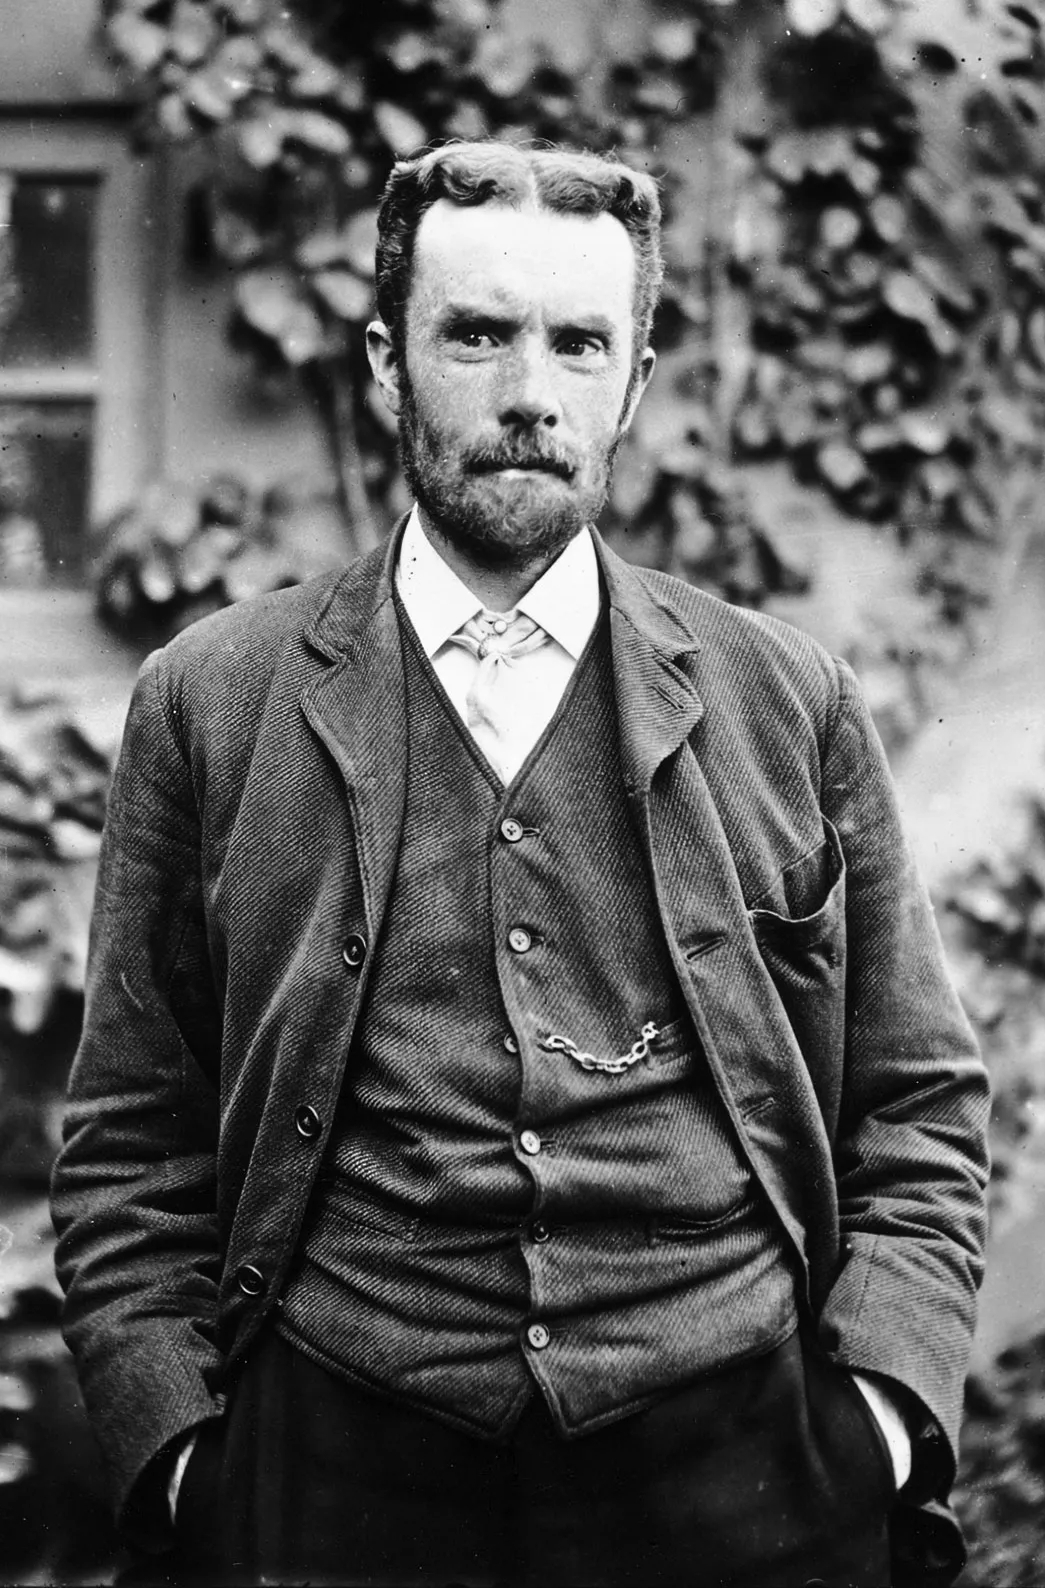
\includegraphics[width=0.3\textwidth]{images/heaviside.jpg}
	
\includegraphics[width=0.6\textwidth]{images/ratigan.jpg}
	\end{figure}

\item {\bfseries\itshape Not enough paper for notes} If you mean my handout, that wasn't meant for notes---just to avoid copying the first page of lecture. If you meant that you ran out of paper, oof. 
 
\item {\bfseries\itshape Will we get a practice test/review before the exam?} I will make an announcement about my recommended study habit for the exam. But, yes, there are old exams that you can try!
\end{itemize}

% 09/04, Thursday: Partial Fractions
\newpage
\section*{09/04, Thursday: Partial Fractions\label{09-04}}

\begin{itemize}
\item {\bfseries\itshape Class Rating:} 8.58/10

\item {\bfseries\itshape Lots of examples was really helpful:} I am glad that you found things helpful! Remember, you can always start the homework right away to make sure that things clicked for you. 

\item {\bfseries\itshape All the examples were helpful:} Great! Always check your understanding by starting the homework!

\item {\bfseries\itshape Very good examples:} Thanks! There are lots of other great ones in the homework\dots \Winkey

\item {\bfseries\itshape Not explaining steps, talking at us rather than teaching:} I do my best to try to explain problems to as many in the class as I can. But like with any class, it definitely is not gonna work for everyone. But feel free to shoutout questions so that I can help clarify things for you!

\item {\bfseries\itshape The pre-lecture was helpful:} Great! Thanks for watching it too!

\item {\bfseries\itshape Good job:} Dziękuję!

\item {\bfseries\itshape Why not just teach us the shortcut?:} As mentioned, the shortcut will not always save us. So, what do we do when it doesn't? We need the long way! So, we cover the long way first so that when we do the shortcut (next time) to save time and it `fails', we can still find the decomposition. Ultimately, the shortcut we shall see is a time saver and not a `solver'. 

\item {\bfseries\itshape Really clear, thank you!:} Thanks! As always, start the homework right away to check your understanding!

\item {\bfseries\itshape Culver's is the best fast food:} Well, we know that's axiomatically wrong because the best fast food is Chipotle, so\dots
	\begin{figure}[H]
	\centering
	
\includegraphics[width=0.3\textwidth]{images/chipotle1.jpg}%
	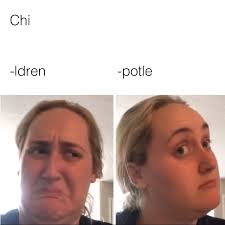
\includegraphics[width=0.31\textwidth]{images/chipotle2.jpeg}%
	
\includegraphics[width=0.39\textwidth]{images/chipotle3.jpg}%
	\end{figure}
\end{itemize}

% 09/02, Tuesday: Trig. Substitution
\newpage
\section*{09/02, Tuesday: Trig. Substitution\label{09-02}}

\begin{itemize}
\item {\bfseries\itshape Class Rating:} 8.54/10

\item {\bfseries\itshape More clear than previous lectures but go too fast when you get on a roll and explain too many steps at a time:} I try to only do/state a single step at a time. But if you're ever confused, don't hesitate to throw out a question! I always post the lecture, so you can also always rewatch the lecture and pause whenever you need more time!

\item {\bfseries\itshape The method for trig sub. was very simple and well explained:} Great! Glad it seemed to click for you. But always remember, following it is one thing, doing it on your own is another. Always check to see what was retained and what will take more time by starting the homework!

\item {\bfseries\itshape How and why are certain trig. functions are chosen over others?:} It depends on how the triangle is set-up. But textbook formulas are given, i.e. the triangles chosen, to avoid the `co-' functions, because their derivatives introduce all sorts of negatives that can cause headaches. You get these substitutions if you force the `vertical' leg to have a variable, if possible. For example, this forces you to choose $x= \sin \theta$, so that $dx= \cos \theta \;d\theta$, compared to $x= \cos \theta$, which forces $dx= -\sin \theta \;d\theta$.

\item {\bfseries\itshape Good job:} Grazie!

\item {\bfseries\itshape This was better than the textbook method:} Thanks! I think so too. Some have started to give a similar presentation, but sadly most have not gone `all the way' with using the triangle. I hope it clicked for you! But this is definitely a tricky method that takes some practice. 

\item {\bfseries\itshape The triangle method and examples were helpful:} Glad things seemed to work for you! But this is definitely a tricky method that takes some practice. So, I would strongly suggest starting the homework soon!

\item {\bfseries\itshape When writing tips/words say what you write as you write it:} I am not sure what parts of the notes you are referring to. Often, I just say it and give ya'll time to copy what I've said. But if I write it, I believe I do say it? It may be a math speak thing, i.e. where we say it a specific way but when we write the math it is written differently. But to us mathematicians, they are `the same' because one representation means the other. Although, I can totally see how this is disconcerting for students.  

\item {\bfseries\itshape I do not know when you apply each method:} That is the hard part of integration. Start to create a list of examples of each type to see what each method might `look like'. For trig. sub., we said explicitly: you are looking for terms that `look like' they could have come from a Pythagorean Theorem, e.g. $x^2 + 4$, $9 - x^2$, etc. 

\item {\bfseries\itshape Comparing everything to triangles made sense:} That's exactly the idea of trig. sub! But this does take some practice, so make sure to try some problems!
\end{itemize}

% 08/28, Thursday: Trigonometric Integrals
\newpage
\section*{08/28, Thursday: Trigonometric Integrals\label{08-28}}

\begin{itemize}
\item {\bfseries\itshape Class Rating:} 8.77/10

\item {\bfseries\itshape Could you post the print out on Blackboard prior to class. The ones you hand out before class. So we can all draw on it on our iPads/computers:} If you mean the note handouts I give you, they are already on Blackboard before the class begins! If you mean the in-class notes, those I am not able to put out before the class starts. In the latter case, they are not pre-written. Otherwise, I would be giving a handout for it. But one trick I have seen students use is that you can hold up your iPad and take a photo with it. You can this drop this photo right into your notes and even write on the photo. I have seen students do nifty things with this. 

\item {\bfseries\itshape The derivative trick for the trig. functions was helpful:} It's still how I remember the derivative of $\tan, \cot, \csc, \sec$. 
	\begin{table}[H]
	\centering
	\begin{tabular}{ccc}
	$\tan$ & $\sec$ & $\sec$ \\
	$\cot$ & $-\csc$ & $\csc$
	\end{tabular}
	\end{table}

\item {\bfseries\itshape I was sleepy:} Me too fam\dots me too\dots

\item {\bfseries\itshape Please continue with the slower pacing with interactive lecture. Thumbs up:} I shall try. But some topics will require more/less discussion in lecture leaving more/less time for a slower pace or more problems. Typically, the more focused problem/question time comes during recitation. 

\item {\bfseries\itshape Was lit:} Bet! Trigonometric integrals be bussin' but we ate that rizz. Drip, DRIP! \dots did I do that right? 

\item {\bfseries\itshape Working through the problems set by step was good. It really helped a lot:} I am glad it helped! But always check that you could do it all on your own later! It's always easier to follow someone thinking it through than it is to do it all yourself. 

\item {\bfseries\itshape Solid class 10/10. Everything was explained and worked out well:} Thanks!

\item {\bfseries\itshape Was easier than recent lessons:} Great! With enough practice, these tend to be among the easiest two or three types of integrals for students that we see in Calc~II. So, get that practice in!

\item {\bfseries\itshape It was hard to see certain exponents:} Sorry! In this case, if I make them too big they start to look like arguments, which really changes how the integral would work, e.g. $\ds\int \sin^2 x \cos^3 x \;dx$ compared to $\ds\int \sin 2x \cos^3 x \;dx$. If you can't make it out, just give a shoutout! I'm happy to clarify. 

\item {\bfseries\itshape Not saying what you are using from step to step, such as power rule, makes lectures confusing, jump from step to step, not giving any formulas either really puts too much stress. Expecting us to memorize integral of everything is crazy:} Most of the steps do not have a precise name. For example, power rule is a derivative rule that is often applied for the corresponding integral, but there are not names for the other elementary integrals, e.g. $\ds\int \tfrac{1}{x} \;dx= \ln|x| + C$. I do try to say what I have done from one step to another---even if I do not write it. But thus far, no formulas! Trigonometric integrals are about a procedure, not a formula. There is no general formula that can be given. Lastly, as for the memorization, every class/field will come with some memorization that has to be done. Even beyond the classroom, eventually, there are just some things you have to know. In principle, you should have learned/memorized these in Calc~I. But if you didn't or forgot them, that's fine! You have plenty of time to slowly let them sink it. In fact, this will happen rather naturally as we use them again and again. So, it's not as daunting as it might seem. Remember, you have the flashcards I handed out to help with them!

\item {\bfseries\itshape It would be nice to have some sort of outline of what we learn in the lecture:} I have done this in the past. I shall try to whip some up for this class too to help make each lecture's learning outcomes clearer.
\end{itemize}

% 08/26, Tuesday: Integration-by-Parts
\newpage
\section*{08/26, Tuesday: Integration-by-Parts\label{08-26}}

\begin{itemize}
\item {\bfseries\itshape Class Rating:} 8.29/10

\item {\bfseries\itshape The slow and concise examples were nice:} Great! Glad it worked for you. But always double check by trying the homework as soon as possible to see what actually made sense and what you need to look at more or ask questions about. 

\item {\bfseries\itshape Not unhelpful just wondering instances where on a looping integral you have two negatives making the original term:} I am not sure what you quite mean by that. But if you're asking about how the signs work out, they work out how they work out. Meaning, if you ended up having $\text{neg} \cdot \text{neg}$, you would get a positive term. If you had $\text{pos} \cdot \text{neg}$, the term would work out negative. It is not the case that the terms `have' to have a certain sign. But the extra $+/-$ added in these products from the `diagonals' in tabular/looping are always the same---alternating positive and negative. 

\item {\bfseries\itshape Is $\ds \int u \;dv= uv \pm ab + \int u \;dv$?:} I think you mean the `formula' for integration-by-parts in the case of a definite integral. This formula is not correct. I think you mean\dots
	\[
	\int_a^b u \;dv= uv \bigg|_a^b - \int_a^b v \;du
	\]

\item {\bfseries\itshape What website/channels are good for outside help? It takes me a little longer than others to grasp the concept of things and get it:} I actually have a whole folder for this on Blackboard! See the `External Resource' folder on Blackboard. You can also stop by my office and ask how I find extra resources. But remember, you also have my/TA office hours, SI sessions, the Math Lab, tutoring, etc. all available to you at USC!

\item {\bfseries\itshape Didn't realize we weren't done with IBP notes and was crashing out over the homework:} We actually covered everything (in principle) you needed to be able to do the integration-by-parts homework by the end of last class. So, if you were having trouble, perhaps it is time to ask for some help! Some struggle is normal and expected, but there is a limit before you should ask for help. So, spend some time on a problem but \textit{never} spend an hour or more on a single problem. Set it aside and come back to it later or ask for help on it!

\item {\bfseries\itshape I appreciated the slow paced examples and explanations\dots:} Happy to hear that everything worked for you!

\item {\bfseries\itshape Tabular integration was only briefly explained:} Even if it was brief, I hope that it was understandable. Maybe it is comforting to know this is typically overwhelmingly the integration technique students do best on after some practice!

\item {\bfseries\itshape This was easy to understand:} Great! But always check your knowledge by trying the homework problems right away!

\item {\bfseries\itshape Can you go a bit slower and write down what you did instead of doing it in your head and writing it. Like how did you get from $\ds -\tfrac{\ln(2x)}{x} + \int \tfrac{1}{x^2} \;dx$ to $-\tfrac{\ln(2x)}{x} - \tfrac{1}{x} + C$:} The only steps I will tend to skip in this course are a simple algebra step (because I trust that even if it takes you a second that you can get it too) or perhaps a linear $u$-substitution. If you're ever stuck on what I did, you can always ask! If you want to figure it out for yourself, you can search for what changed from one step to another. Notice the only thing different is the integral went away. I must have integrated! Indeed, the only thing I did was integrate $\ds\int \tfrac{1}{x^2} \;dx= -\tfrac{1}{x} + C$. While I said this step, I did not write it. Never hesitate to ask if you're unsure of how I got from one step to another!

\item {\bfseries\itshape Why do you set the looping ones equal to the original integral?:} The idea is we have an integral, say $\ds\int e^x \sin x \;dx$. We do some integration-by-parts (in this case twice) and then have\dots
	\[
	e^x \sin x - e^x \cos x - \int e^x \sin x \;dx
	\]
The problem is that we wanted to find out how to compute $\ds\int e^x \sin x \;dx$, and now we just have to figure out\dots $\ds\int e^x \sin x \;dx$. We have looped back to the original! So, what are we supposed to do? If we remember that we started with $\ds\int e^x \sin x \;dx$, what we found above is equal to this integral (hence setting equal to the original integral):
	\[
	\int e^x \sin x \;dx= e^x \sin x - e^x \cos x - \int e^x \sin x \;dx
	\]
How did this help us? Notice if we add $\ds\int e^x \sin x \;dx$ to both sides, on the right side it cancels but on the left we get twice the integral---just like how $x + x= 2x$. But then\dots
	\[
	2\int e^x \sin x \;dx= e^x \sin x - e^x \cos x
	\]
So, if we divide by 2, we can find the integral!
	\[
	\int e^x \sin x \;dx= \dfrac{e^x \sin x - e^x \cos x}{2} + C
	\]
This type of `trick' is exactly the idea of `looping' integrals. 

\item {\bfseries\itshape Explain each part, we are in summer mode you tend to skip \underline{important} small steps out of habit:} I never skip actually important steps. But, for sure, I will skip small algebra steps or things like that. It is fine if you need a few more seconds or a minute on something like that. The important thing is not that you do it `instantly' in your head, but rather that you \textit{can} get there. But if I had to show everything down to last algebra steps, we would not be able to cover everything or have greatly reduced examples. It's a trade off---but one I feel is worth it. But I totally get how this can be frustrating. Remember, you can always play the lecture back and pause to do things in your own time! 

\item {\bfseries\itshape I don't even know, I'm kind of just confused on everything:} Oof. I am sorry to hear that. It can be tough to keep pace with class at times. Lectures speak to the room, but when you come to office hours (either for me or the TA), attend SI sessions, get tutoring, etc., you have someone speaking specifically to you, which can be much easier. So, don't hesitate to stop by/reach out! There's lots of support for you. You got this!

\item {\bfseries\itshape Thanks for making things simple:} No problem. But remember, even with the shortcuts, you need to practice!

\item {\bfseries\itshape The tabular/looping integrals were well explained:} Thanks! Be sure to try a few to make sure that you are able to do it! With enough practice, these tend to be a type of integral students are really good at! So, putting in the practice with these can really pay off!

\item {\bfseries\itshape I felt that we jumped into a topic that we didn't even start the class before:} Yes and no. It was still integration-by-parts. But this class was about a shortcut in two special cases. So, other than the fact we are still using LIATE, this was indeed a topic we did not see last class!

\item {\bfseries\itshape Good job:} Gracias!

\item {\bfseries\itshape Your handwriting can be confusing:} I am sorry. I have been told that I have `flowery' handwriting. I shall try to write larger, which will hopefully make that clearer. But if you can't read something, feel free to shout out asking what it is!

\item {\bfseries\itshape It was helpful to take time to explain when to use what:} No problem! Just make sure that you know when something is `normal' integration-by-parts, when it is `tabular', and when it is `looping'. 

\item {\bfseries\itshape I think you explained it well and slower:} Thanks! Remember, it is best to try the homework right away so that you can see what actually ended up sinking in and what you need more time with or might need to ask for help with!

\item {\bfseries\itshape Why do you think One Piece is bad (don't say pacing)?:} Oh, so you mean ignoring the reason that makes a show bad, why is the show bad? {\itshape *snap*} You know One Piece has more episodes than Naruto (in its entirety, including filler), DragonBallZ, and Attack on Titan \textit{combined}, right? Has it really covered enough with its time to be worth the time? Keep in mind, with that time, you could have watched all those shows\dots {\itshape *snaps slowly, like One Piece*}
\end{itemize}

% 08/21, Thursday: Integration-by-Parts
\newpage
\section*{08/21, Thursday: Integration-by-Parts\label{08-21}}

\begin{itemize}
\item {\bfseries\itshape Class Rating:} 8.45/10

\item {\bfseries\itshape It was nice to be shown examples and then to try ourselves:} I am glad that this lecture clicked more for you. I honestly try to build in as much `try it yourself' time as possible. But some lectures will have more/less of that depending on the topic. The real `do problems' time is recitation. 

\item {\bfseries\itshape The box method was helpful:} Glad you liked it. But even if it felt like it `clicked', always remember to get to the homework asap to see if it actually did. If it didn't, then you have a chance to put things on track before we dive further. Remember, it's easier (but not necessarily easy) to keep up than to catch up!

\item {\bfseries\itshape Towards the end it got complicated:} That was actually kind of the point! Those last two examples---$\ds\int x^2 e^x \;dx$ and $\ds\int e^x \sin x \;dx$---were definitely harder than the others. For the former, we had to use integration-by-parts twice. For the second, it somehow `looped' back on itself. They were awful! We did need to see the `long way'. Finding ways of avoiding having to do these integrals this way would be great\dots and is the point of the next lecture! 

\item {\bfseries\itshape It was a lot to absorb all at once:} Some lectures will be like that. Not everything is going to come right away; that's fine and natural. Remember, you can rewatch the lecture and pause at your own pace. You can also stop by to ask me or the TA questions. You can also ask the SI to help clarify points!

\item {\bfseries\itshape Have a hard time seeing the problems:} I will try to write larger and/or zoom in more!

\item {\bfseries\itshape The pacing was better today:} Great that things went smoother for you! But remember, it is always easier to follow in lecture than it is 100\% own your own. So, try the homework to see what `settled in' and what you might need to look at more!

\item {\bfseries\itshape It would be nice to know what you expect from us when solving a problem. Like the `7' method, it was kind of very quickly explained yet then we had to do a problem:} Calculus~II is all about doing problems! Though it seems like some kind of shortcut (and it is), everything I showed was everything you need to show for the `7'-method---no more or less. So, if you did those problems as I did in-class on the exam, you'd be perfectly fine!

\item {\bfseries\itshape love the 7:} It always felt like a casino type deal---777. 

\item {\bfseries\itshape I need more clarification on when to use $u$-sub. and when to use IBP:} That \textit{is} the hard part. Both $u$-substitution and integration-by-parts are \textit{very} general methods that apply to many types of integrals. The eventual goal is to be able to look at an integral and have a `feel' for what method might be best. Eventually, we will have methods that apply to specific types of integrals. So, once we have those, it is easier to work from these more specific methods `backwards' to the most general in order to figure out what approach might be best. Indeed, it is not always easy to see which types of integrals `require' $u$-substitution or integration-by-parts. But with enough problems under your belt, you will get a feel for this!

\item {\bfseries\itshape Super cool stuff:} Just wait to see the other tricks that we get to see!

\item {\bfseries\itshape Please zoom in and write bigger please. Find a way to have the iPad fill screen:} I shall try. It is a battle. If you zoom in a lot, things are bigger but then you have to move about more and not everything is on the screen. It's then easy for students to fall behind or miss writing things that are no longer on the screen. It's a balancing act and I shall do my best. 

\item {\bfseries\itshape Solid!:} Danke!

\item {\bfseries\itshape It was helpful to have some problems to do:} And there's lots more to be seen on the homework \Laughey
\end{itemize}

% 08/19, Tuesday: u-Substitution Review
\newpage
\section*{08/19, Tuesday: $u$-Substitution Review\label{08-19}}

\begin{itemize}
\item {\bfseries\itshape Class Rating:} 8.51/10

\item {\bfseries\itshape The 2nd type of $u$-sub was least helpful:} I think you mean the `hoity-toity'/`in-place' method compared to just substituting. While it can definitely feel `weirder' than the approach you might have been taught at first, this `in-place' approach is actually easier for certain types of integrals, e.g. trigonometric integrals, that we will see later. So, it is important that we get a feel for it now to make things easier for us down the line. But for sure, it takes some practice. 

\item {\bfseries\itshape We moved very fast:} We will have to move faster in some classes than others to cover everything. So, some classes will be slower or have more time for some in-class practice. Of course, today we moved a bit faster because---in theory---everything from today should have been review! If you couldn't quite remember everything, that's perfectly fine! You just came from a long summer. It's perfectly natural to have forgotten some things. But hopefully, after covering so much today, you have a feel for what you remember and what you need to review. 

\item {\bfseries\itshape Most helpful was the linear $u$-sub.:} I am glad that you found it helpful! Remember, you will want to practice this until you get a feel for it enough to be able to do it in your head. This makes the future integrals \textit{much} easier to deal with. 

\item {\bfseries\itshape Good job:} Thanks! 

\item {\bfseries\itshape Would you recommend Pearson+?:} I do not know anything about Pearson+. I cannot imagine it would have more resources than what you could find on Blackboard per topic. So, I would recommend whatever is the cheapest option for Pearson. 

\item {\bfseries\itshape It would help if class notes could be online so I can use my iPad:} If you mean the note handouts I give you, they are already on Blackboard before the class begins! If you mean the in-class notes, those I am not able to put out before the class starts. In the latter case, they are not pre-written. Otherwise, I would be giving a handout for it. But one trick I have seen students use is that you can hold up your iPad and take a photo with it. You can this drop this photo right into your notes and even write on the photo. I have seen students do nifty things with this. 

\item {\bfseries\itshape I accidentally sat in on the wrong class :( :} Oof. You didn't need to stay in a class that you aren't enrolled in! It's easy to get lost the first day. Definitely, don't stay in a class you aren't in. It's no problem to get up and find your actual class. You don't want to miss the first day! \dots but then I realize you'll never read this\dots oh.

\item {\bfseries\itshape You explained too much and too little:} I will do my best to try to `Goldilocks' that next time. 

\item {\bfseries\itshape Wish we did the syllabus:} We did! I covered it in a syllabus video posted to Blackboard and asked if there were any questions on it! This saved us a full class, which we can then spend to give us an extra lecture on one of the future integration techniques. I think that in the long-run, you'll much prefer this over talking about the syllabus! 

\item {\bfseries\itshape Have trouble seeing what's written:} I will do my best to write larger/zoom in more.

\item {\bfseries\itshape The note packet was really helpful:} Thanks! Remember, if you ever lose it or need another copy, everything is linked in Blackboard. So, there is a master set of notes you can print (full-size even) the notes that I handed out. 
\end{itemize}

\end{document}